



\subsection{Orthogonal Projections}
\begin{frame}{Orthogonal projections}
\begin{itemize}
\item A \textit{line} spanned by a vector $u$ is the set of all multiple vector of $u$. That is
\begin{align*}
    l_u = \{ v\mid  v = \lambda u \;\text{ for some } \; \lambda \in \mathbb{R}\} := span \left\{ u\right\}
\end{align*}
\item A plan spanned by two vectors $u,v$ is the set of all  linear combination of $u$ and $v$; that is 
\begin{align}
    \pi_{uv} = \left\{\lambda u + \beta v \mid \lambda, \; \beta\in \mathbb{R} \right\} := span \left\{ u,v\right\}
\end{align}
\item Example: 
\begin{align*}
    \mathbb{R}^2 = \{\lambda e_1 + \beta e_2 \mid \lambda, \beta\in \mathbb{R} \}
\end{align*}
\end{itemize}
\end{frame}

\begin{frame}{Projection onto a line}
\begin{itemize}
    \item \textbf{Projection of a vector onto a line}: if a $x$ is a vector, the projection $p$ of $x$ on a line spanned by $u$ is  defined as 
    \begin{align}
        p = \frac{x^T u}{\Vert u \Vert ^2}u
    \end{align}
    \item We call $e=u-p$ the error and satisfies $u^Te=0$.
    \item \textbf{Projection matrix}  If we denote $\hat{p}=\frac{x^Tu}{\Vert u \Vert^2}$,we can write $p$ as $p=Px$, where $P$ is the projection matrix given as  
    \begin{align}
        P = \frac{uu^T}{\Vert u \Vert^2} 
    \end{align}
 \end{itemize}
\end{frame}
\begin{frame}{}
\begin{center}
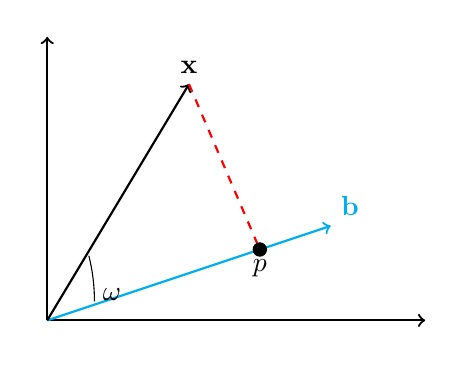
\begin{tikzpicture}[scale=1.2]
    % Origin
    % Axes
    \draw[->, thick] (0,0) -- (4,0) node[below] {};
    \draw[->, thick] (0,0) -- (0,3) node[left] {};
    
    % Basis vector b (yellow arrow)
    \draw[->, thick, cyan] (0,0) -- (3,1) node[above right] {$\mathbf{b}$};
    
    % Vector x (black arrow)
    \draw[->, thick] (0,0) -- (1.5,2.5) node[above] {$\mathbf{x}$};
    
    % Projection of x onto b (red dashed line)
    \draw[dashed, red, thick] (1.5,2.5) -- (2.25,0.75);
    
    % Projected point on b
    \filldraw[black] (2.25,0.75) circle (2pt) node[below] {$p$};
    
    % Angle omega between b and x
    \draw (0.5,0.2) arc (0:14:2) node[midway, below right] {$\omega$};
\end{tikzpicture}
\end{center}
\begin{itemize}
\item Example: Suppose $x$ and $u$ are given as 
    \begin{align*}
        x = \begin{bmatrix}
            2\\3
        \end{bmatrix}, \; u =\begin{bmatrix}
            1\\0
        \end{bmatrix}
    \end{align*}
    \item $\Vert u \Vert ^2 = 1$
    \item $x^T u = 2\times 1 + 3\times 0 = 2$
\end{itemize}
\end{frame}
\begin{frame}{}
\begin{itemize}
    \item $p= 2\begin{bmatrix}
        1\\0
    \end{bmatrix}= \begin{bmatrix}
        2\\0
    \end{bmatrix}$
    \item Find the projection matrix $P$ onto a line through the origin spanned by $b=[1, 2, 2]$. We have:
    \begin{align}
        P = \frac{bb^T}{\Vert b \Vert ^2} = \frac{1}{9} \begin{bmatrix}
            1\\ 2\\ 2 
        \end{bmatrix}\begin{bmatrix}
            1 & 2& 2 
        \end{bmatrix} = \frac{1}{9} \begin{bmatrix}
            1 & 2&2\\
            2&4 & 4\\
            2&4&4
        \end{bmatrix}
    \end{align}
    \item Now, given any vector $x$, its projection onto the line spanned by $b$ is given as 
    \begin{align}
        p = Px = \frac{1}{9} \begin{bmatrix}
            1 & 2&2\\
            2&4 & 4\\
            2&4&4
        \end{bmatrix}\begin{bmatrix}
            x_1\\x_2 \\
            x_3
        \end{bmatrix}
    \end{align}
\end{itemize}
\end{frame}
\begin{frame}{Exercice}
\begin{enumerate}
    \item Find the projection vector $p$ and give the projection matrix $P$ for the following vectors:
    \begin{align}
        a)\;\; x=\begin{bmatrix}
        1\\1\\1
    \end{bmatrix}, \;u=\begin{bmatrix}
        1\\2\\2
    \end{bmatrix}\;\; b) \;\;  x=\begin{bmatrix}
        1\\0\\1
    \end{bmatrix}, u=\begin{bmatrix}
        1\\-1\\2
    \end{bmatrix}
    \end{align}
    \item For each case above,  compute $P^2$ and $P^3$. What do you observe?
    \item  Show that the error $e=u-p$ is perpendicular  to $u$, i.e. $u^Te=0$
    \item show that $\Vert p \Vert = \Vert b \Vert \cos \theta$, where $\theta$ is the angle between $p$ and $b$.
\end{enumerate}
\end{frame}

\begin{frame}{}
\begin{itemize}
    \item \textbf{Projection of a vector onto a plan}: Given a vector $x$ and a $2-D$ plan $\pi$.  The projection of $x$ onto $\pi$, it is a vector $x^{'}$ given by
    \begin{align}
        x^{'} = \frac{x^Tu}{\Vert u \Vert^2}u + \frac{x^Tv}{\Vert v \Vert ^2}v
    \end{align}
    \item In matrix notation, the project of  $x^{'}$ of $x$ is:
    \begin{align}
        x^{'} = \left( I - nn^T \right) x,
    \end{align}
    where $n$ is the normal unit vector, and $P = I -nn^T$ the orthogonal projection matrix.
\end{itemize}
\end{frame}
\begin{frame}{}
\begin{figure}
\begin{center}
    \begin{tikzpicture}[scale=1.5]
    % Define the parallelogram (plane) vertices
    \coordinate (A) at (0,0,0);
    \coordinate (B) at (3,0,0);  % Adjust for the slant of the parallelogram
    \coordinate (AB) at (1,0,0)node[below]{$O$}
    \coordinate (AD) at (0.3,1,-1);
    \coordinate (C) at (4,2,0);  % Adjust for the shape
    \coordinate (D) at (1,2,0);  
    \draw (2,0,0)node[below]{$u$};
    \draw (0.3,1,-1)node[left]{$v$};
    
    % Draw the parallelogram (plane)
    \draw (A) -- (B) -- (C) -- (D) -- cycle;
    \draw [->, thick](A) -- (AB);
    \draw[->, thick] (A)--(AD);
    
    % Label the corners of the parallelogram
    \node[below left] at (A) ;
    \node[below right] at (B) ;
    \node[above right] at (C) ;
    \node[above left] at (D) ;
    
    % Define the perpendicular line (normal to the plane) starting from the center of the parallelogram
    \coordinate (Center) at (2,1,0);  % Approximate center of the parallelogram
    \draw (2,3,0) node[above right]{x};
    \draw[->, very thick, red] (O) --(2,3,0);
    \draw[->, very thick, cyan] (O)-- (2,1,0);
    \draw[dashed] (2,3,0) -- (Center)node[midway, right]{$x-x^{'}$};
    \coordinate (Top) at (2,1.5,2);  
    \draw (2,1.4,0)--(2.2,1.4,0)--(2.2,1,0);
    \draw (2,1,0)node[below]{$x^{'}$};
\end{tikzpicture}
  \caption{Projection onto a plan spanned by $u$ and $v$. The projection $x^{'}$ can be expressed as a linear combination of $u$ and $v$ and the displacement vector $x-^{'}$ is orthogonal to $u$ and $v$.}
    \label{fig:enter-label}
\end{center}
\end{figure}
\end{frame}
\begin{frame}{}
    \begin{itemize}
        \item Example:  Suppose the normal vector $n$ and the vector $u$ are 
        \begin{align*}
            n = \begin{bmatrix}
                0\\0\\1
            \end{bmatrix}, \; x = \begin{bmatrix}
                1\\2\\3
            \end{bmatrix}
        \end{align*}
        \item We should first ensure that $n$ is a unit vector, that is $\Vert n \Vert =1$, which is  already the case.
        \item Compute $nn^T$: 
        \begin{align*}
            nn^T = 
                \begin{bmatrix}
                0\\0\\1
            \end{bmatrix}[0\; 0\; 1] = \begin{bmatrix}
                0 &0& 0\\
                0&0& 0\\
                0&0&1
            \end{bmatrix},
        \end{align*}
        \item The project matrix $P$: 
    \end{itemize}
\end{frame}
\begin{frame}{}
\begin{itemize}
     \item The project matrix $P$: 
     \begin{align*}
         P = I -nn^T = \begin{bmatrix}
             1&0&0\\
             0&1&0\\
             0&0&1
         \end{bmatrix} - \begin{bmatrix}
                0 &0& 0\\
                0&0& 0\\
                0&0&1
            \end{bmatrix}= \begin{bmatrix}
                1 & 0 & 0\\
                0& 1& 0 \\
                0& 0& 0
            \end{bmatrix}
     \end{align*}
     \item Project $x$:
     \begin{align*}
         x^{'} = Px = \begin{bmatrix}
                1 & 0 & 0\\
                0& 1& 0 \\
                0& 0& 0
            \end{bmatrix}\begin{bmatrix}
                1\\2\\3
            \end{bmatrix} = \begin{bmatrix}
                1\\2\\0
            \end{bmatrix}
     \end{align*}
\end{itemize}
\end{frame}